\section{Systemopbygning}
For at kunne finde krav til dette projekts HiFi-forstærker er det nødvendigt at vælge hvilke blokke denne skal bestå af. I dette projekt er der ikke udelukkende valgt at designe en HiFi-forstærker i sin simpleste form, men også at tilføje funktionalitetsudvidende elementer. Systemets opbygning, med adskilte funktionelle blokke, er illustreret på figur \ref{fig:hififorstaerker_opbygning}. Dette afsnit vil argumentere og forklare den valgte opbygning. 


\begin{figure}[h]
\centering
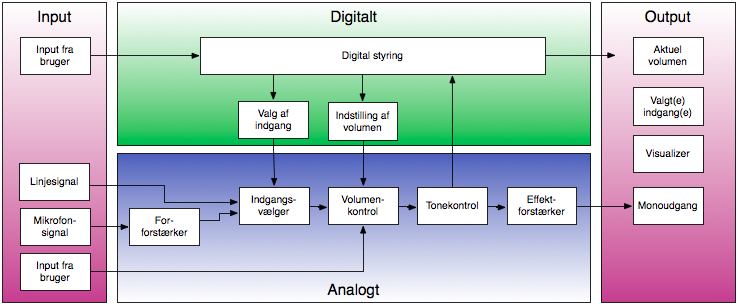
\includegraphics[scale=0.6]{indledende_analyse/systemopbygning/forstaerker_opbygning.png}
\caption{Opbygning af dette projekts HiFi-forstærker}
\label{fig:hififorstaerker_opbygning}
\end{figure}


\subsection*{Input blokke}
Det er valgt at der skal kunne tilsluttes to typer lydkilder til HiFi-forstærkeren; en mikrofon og en kilde som afgiver et liniesignal. Kilder som afgiver et liniesignal er blandt andre computere, de fleste mobiltelefoner og medieafspillere, hvilket er grundlaget for netop at vælge denne type indgang. 
Grundlaget for at vælge en mikrofonindgang er udelukkende for at kunne anvende en indgangsvælger og for ikke at lave to ens linjeindgange. Desuden præsenterer en mikrofonindgang en ny blok: forforstærker.

HiFi-forstærkeren skal udstyres med et frontpanel hvorpå alle knapper til justeringsmulighederne skal placeres, således at de er tilgængelige for brugeren. Justeringsmulighederne, som skal være tilgængelige for brugeren er equalizerbånd, volumen og valg af indgang.

\subsection*{Analoge blokke}

Udgangsspændningen fra en mikrofon er langt lavere end linieniveau. Derfor benyttes en forforstærker til at forstærke mikrofonens lave signal op på niveau med liniesignalet, således at de er sammenlignelige i resten af systemet.

For at kunne vælge 

Forforstærker
Indgangsvælger
Volumenkontrol
Tonekontrol
Effektforstærker

\subsection*{Digital styring}
Digital styring


\subsection*{Output blokke}
Displays
Monoudgang